\documentclass[conference]{IEEEtran}
\IEEEoverridecommandlockouts
% The preceding line is only needed to identify funding in the first footnote. If that is unneeded, please comment it out.
\usepackage{cite}
\usepackage{amsmath,amssymb,amsfonts}
\usepackage{algorithmic}
\usepackage{graphicx}
\usepackage{textcomp}
\usepackage{xcolor}
\def\BibTeX{{\rm B\kern-.05em{\sc i\kern-.025em b}\kern-.08em
    T\kern-.1667em\lower.7ex\hbox{E}\kern-.125emX}}

\begin{document}

\title{Practical Work I - Report\\
{\footnotesize \textsuperscript{}This report has been carried out for the ANADI Curricular Unit}
}

\author{
\IEEEauthorblockN{1\textsuperscript{st} Francisco Redol}
\IEEEauthorblockA{\textit{Instituto Politécnico do Porto} \\
\textit{ISEP - DEI}\\
Porto, Portugal \\
1201239@isep.ipp.pt}
\and

\IEEEauthorblockN{2\textsuperscript{nd} Mariana Lages}
\IEEEauthorblockA{\textit{Instituto Politécnico do Porto} \\
\textit{ISEP - DEI}\\
Porto, Portugal \\
1200902@isep.ipp.pt}
\and

\IEEEauthorblockN{3\textsuperscript{rd} Miguel Jordão}
\IEEEauthorblockA{\textit{Instituto Politécnico do Porto} \\
\textit{ISEP - DEI}\\
Porto, Portugal \\
1201487@isep.ipp.pt}
}

\maketitle

\begin{abstract}
On this report, we utilized R language features to support our affirmations and conclusions.
Themes such data analysis, data modeling and non/parametric tests were used on the data
from imported .csv files. 
\end{abstract}

\begin{IEEEkeywords}
regression, data analysis, data modeling, R language
\end{IEEEkeywords}

\section{Introduction}

Exploratory analysis is elected as the first step in a data analysis process, providing insights into a dataset's characteristics. By exploring and summarizing data through numerous statistical and graphical procedures, researchers can identify patterns, anomalies, and potential outliers, which can guide further analysis and hypothesis testing, along with formulating theories around a certain subject. 
In this research, we will discuss key statistical aspects of that character, such as exploratory analysis, parametric and non-parametric tests, linear regression, and data modelling based on the provided datasets. 
By giving an insight into these techniques and their applications, we aim to emphasise the importance of these backbone concepts while doing scientific research.
In the proposed assignment, there are three distinct datasets which will be thoroughly described, along with the steps to dissect these.

\subsection{Vehicles Dataset - Data Treatment}
The "Dados3.csv" dataset contains data about vehicle characteristics, such as acceleration, the number of cylinders in the engine, along with horsepower and the vehicle's weight.
Through exploratory analysis, given more context, it is possible to find hidden to the naked eye information, allowing a deeper understanding of a certain context.
For instance, a brand or a specific model.
\section{Exploratory Analysis - Vehicles}
Since the exercise requests to examine if there are significant differences in acceleration values between the three engine cylinder groups, it is pivotal to partition the acceleration values according to the number of cylinders. 
This is required because the proposed challenge questions if there are significant differences in the acceleration between vehicles, which leads to a concrete hypothesis test, allowing us to answer this question through the provided accelerations per cylinder.
So, two hypotheses were synthesized:
    \begin{itemize}
        \item H0: There aren't significant differences between acceleration values according to the cylinder count;
        \item H1: There are significant differences between acceleration values between the distinct groups.
    \end{itemize}
After formulating the two possible premises, we observe that the faced test is bilateral.
This is due to us facing an interest in solely finding out whether the mean acceleration of one group is higher or lower than the other one.\\

To prepare the data for the performed analysis, we first imported the dataset, which then was segregated into three distinct categories. 
These are the different numbers of cylinder counts: 4, 6 and 8.\\

After setting up the required data, for the trial to be started, we needed to evaluate which kind of test could be performed on this population. 
Starting with ANOVA, there are 6 exclusive steps which need to be accomplished.\\

First, is the dependent variable continuous? Because it varies according to the number of cylinders and takes infinite possibilities of values within a certain range, it is considered so.

Second, the independent variable (number of cylinders) has 3 groups of values, which complies with the two or plus variable groups.

Third, the observations are independent, considering that according to the essay, the number of cylinders is the key factor to consider in this variation.

Fourth, do the observations have significant outliers? To answer this question, a boxplot (a type of graphic that displays the median, quartiles, and outliers of the data) was generated.\\

\begin{figure}[htbp]
    \centering{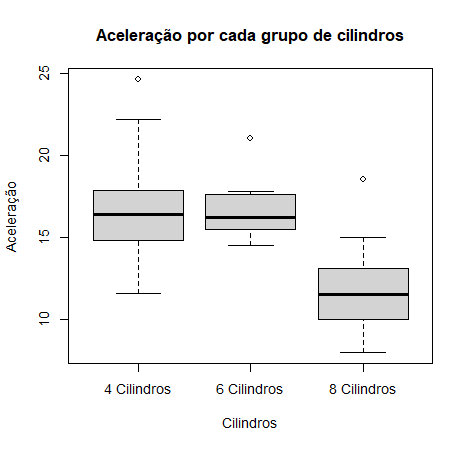
\includegraphics[width=5cm]{images/vehicles/boxplot.png}}
    \caption{Boxplot of the acceleration values according to the number of cylinders.}
    \label{vehicle_boxplot}
\end{figure}

At first sight, the results demonstrate that the 4-cylinder group has the highest median acceleration value (16.4), closely followed by the 6-cylinder group (16.2), 
which pulls a significant distance from the 8-cylinder engines acceleration (11.5). 
It is obvious that the interquartile range on 4 and 8-cylinders is much ampler than the 6-cylinders. 
Its whiskers are also much more wide-ranging. 
Diving deeper into the quartiles analysis, for 4-cylinder powered vehicles, the quartile inferior limit is 10.2, with its superior limit around 22.4, close to the represented outlier. 
For the 6-cylinder, the inferior and superior limits were 12.3 and 20.8, respectively. 
Lastly, on the 8-cylinder designed cars, 5.35 and 17.8. 

After closely observing the boxplot it is confirmed that significant outliers exist, considering that acceleration is a continuous variable. 
These are random points outside of the whiskers(highest and lowest observations within 1.5 times the interquartile range), particularly important when applied to a real-life scenario. 
They could be explained by a vast number of variables, for instance, tyre pressure, which is outside of our scope. 
Outliers are one of the most interesting/curious parts of a boxplot since they can reveal hidden causes.\\

However, it is clear that 6-cylinder cars produce much more consistent results, while the remaining two have a wider spectre of traduced power.



























\section*{References}

Please number citations consecutively within brackets \cite{b1}. The 
sentence punctuation follows the bracket \cite{b2}. Refer simply to the reference 
number, as in \cite{b3}---do not use ``Ref. \cite{b3}'' or ``reference \cite{b3}'' except at 
the beginning of a sentence: ``Reference \cite{b3} was the first $\ldots$''

Number footnotes separately in superscripts. Place the actual footnote at 
the bottom of the column in which it was cited. Do not put footnotes in the 
abstract or reference list. Use letters for table footnotes.

Unless there are six authors or more give all authors' names; do not use 
``et al.''. Papers that have not been published, even if they have been 
submitted for publication, should be cited as ``unpublished'' \cite{b4}. Papers 
that have been accepted for publication should be cited as ``in press'' \cite{b5}. 
Capitalize only the first word in a paper title, except for proper nouns and 
element symbols.

For papers published in translation journals, please give the English 
citation first, followed by the original foreign-language citation \cite{b6}.

\begin{thebibliography}{00}
\bibitem{b1} G. Eason, B. Noble, and I. N. Sneddon, ``On certain integrals of Lipschitz-Hankel type involving products of Bessel functions,'' Phil. Trans. Roy. Soc. London, vol. A247, pp. 529--551, April 1955.
\bibitem{b2} J. Clerk Maxwell, A Treatise on Electricity and Magnetism, 3rd ed., vol. 2. Oxford: Clarendon, 1892, pp.68--73.
\bibitem{b3} I. S. Jacobs and C. P. Bean, ``Fine particles, thin films and exchange anisotropy,'' in Magnetism, vol. III, G. T. Rado and H. Suhl, Eds. New York: Academic, 1963, pp. 271--350.
\bibitem{b4} K. Elissa, ``Title of paper if known,'' unpublished.
\bibitem{b5} R. Nicole, ``Title of paper with only first word capitalized,'' J. Name Stand. Abbrev., in press.
\bibitem{b6} Y. Yorozu, M. Hirano, K. Oka, and Y. Tagawa, ``Electron spectroscopy studies on magneto-optical media and plastic substrate interface,'' IEEE Transl. J. Magn. Japan, vol. 2, pp. 740--741, August 1987 [Digests 9th Annual Conf. Magnetics Japan, p. 301, 1982].
\bibitem{b7} M. Young, The Technical Writer's Handbook. Mill Valley, CA: University Science, 1989.
\end{thebibliography}
\vspace{12pt}
\color{red}
IEEE conference templates contain guidance text for composing and formatting conference papers. Please ensure that all template text is removed from your conference paper prior to submission to the conference. Failure to remove the template text from your paper may result in your paper not being published.

\end{document}
